
             \newcommand{\textonecolor}[1]{\ifnum2<#1black\else black!50\fi}
  \only<2>{\renewcommand{\textonecolor}[1]{\ifnum3<##1black\else black!50\fi}}
  \only<4>{\renewcommand{\textonecolor}[1]{\ifnum4<##1black\else black!50\fi}}

             \newcommand{\nodeonecolor}[1]{\if3#1red!20\else none\fi}
  \only<2>{\renewcommand{\nodeonecolor}[1]{\if4##1red!20\else none\fi}}
  \only<4>{\renewcommand{\nodeonecolor}[1]{\if5##1red!20\else none\fi}}
  \begin{center}
    \begin{tikzpicture}[]

      \def \n {6}
      \def \radius {3}
      \def \margin {15} % margin in angles, depends on the radius

      \foreach \s/\t in {1/Purpose,2/Research,3/Hypothesis,4/Experiment,5/Analysis,6/Conclusion}
      {
        \node[fill=\nodeonecolor{\s},text=\textonecolor{\s},circle,minimum width=3] at ({360/\n * (\s - 1)}:\radius) {\t};
        \draw[->, >=latex] ({360/\n * (\s - 1)+\margin}:\radius) 
        arc ({360/\n * (\s - 1)+\margin}:{360/\n * (\s)-\margin}:\radius);
      }
    \end{tikzpicture}
    \addtooverlay<.(3)>{%
      \draw[fill=black,opacity=1.00] 
      (current page.north east) rectangle (current page.south west);
      \node at (current page.center) {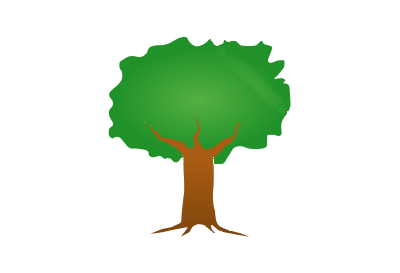
\includegraphics[height=\textheight]{media/tree.png}};
    }
  \end{center}
